\documentclass{beamer}
\hypersetup{pdfstartview={Fit}}

\usepackage[french]{babel}
\usepackage[T1]{fontenc}
\usepackage[utf8]{inputenc}

\usepackage{amsmath}
\usepackage{amssymb}
\usepackage{amsthm}

\usepackage{tikz}

\usepackage{wrapfig}

% quelques définitions
\theoremstyle{plain}
\newtheorem{thm}{Théorème}
\newtheorem{prop}{Proposition}

\theoremstyle{definition}
\newtheorem{defi}{Définition}
\newtheorem{qst}{Question}
\newtheorem{rmq}{Remarque}

\DeclareMathOperator\Var{Var}
\DeclareMathOperator\Cov{Cov}


\usetheme{Montpellier}
\usecolortheme{whale}
\beamertemplatenavigationsymbolsempty

\title{Reconnaissance faciale par Eigenfaces}
\author{Bouarah Romain \and Langdorph Matthieu \and Ketels Lucas \and Nathan Souffan }
\date{\today}

\begin{document}


\begin{frame}[plain]
  \titlepage
\end{frame}


\begin{frame}[plain]
  \tableofcontents
\end{frame}

\section{Calcul des eigenfaces}
\subsection{Travail dans $\mathbb{R}^{N \times N}$}
\begin{frame}
  \frametitle{Représentation matricielle des images}
  \begin{defi}
    Une image de taille $N \times N$ est représentée par une matrice $N \times N$.\\
    Chaque coefficient représente un niveau de gris d'un pixel.
  \end{defi}
\end{frame}



\begin{frame}
  \frametitle{Transformation en un vecteur de $\mathbb{R}^{N \times N}$}
  On juxtapose simplement les colonnes de la matrice l'une en dessous de l'autre.
  \[
    \begin{pmatrix}
      p_{1,1} & p_{1,2} & \cdots & p_{1,N} \\
      p_{2,1} & p_{2,2} & \cdots & p_{2,N} \\
      \vdots  & \vdots  & \ddots & \vdots  \\
      p_{N,1} & p_{N,2} & \cdots & p_{N,N}
    \end{pmatrix}
    \rightarrow
    \begin{pmatrix}
      p_{1,1} \\
      p_{2,1} \\
      \vdots \\
      p_{N,1} \\
      \vdots \\
      p_{1,N} \\
      \vdots \\
      p_{N,N}
    \end{pmatrix}
  \]  
\end{frame}



\subsection{Matrice de covariance}



\begin{frame}  
  \frametitle{Observation sur les images des visages}
  \begin{qst}
    Que dire de la position de nos images de visages dans l'espace $\mathbb{R}^{N \times N}$?
  \end{qst}
  \pause
  \begin{exampleblock}{Réponse}
    Nos images de visages ne sont pas si éloignées les unes des autres. 
  \end{exampleblock}
\end{frame}



\begin{frame}
  \frametitle{Définition de la Matrice de Covariance}  
  \begin{defi}
    La matrice de covariance d'un vecteur de $p$ variables aléatoires $\overrightarrow{X} =
    \begin{pmatrix}
      X_1 \\
      \vdots \\
      X_p
    \end{pmatrix}$ dont chacune possède une variance, est la matrice carrée dont le terme générique est donné par $a_{i,j} = \Cov(X_i,X_j)$.
  \end{defi}
\end{frame}



\begin{frame}
  \frametitle{Encodons cette dispersion}  
  \begin{defi}[Estimation de la Matrice de Covariance]
    En partant d’un échantillon de réalisations indépendantes d’un vecteur aléatoire, une estimation de la matrice de covariance est donné par :
    \[
      \Var(\overrightarrow{X}) = \frac{1}{n} \displaystyle\sum_{i=1}^{n} (\overrightarrow{X_i} - \overrightarrow{\mu})(\overrightarrow{X_i}-\overrightarrow{\mu})^T
    \]
    où $\overrightarrow{\mu} = \frac{1}{n} \displaystyle\sum_{i=1}^{n}\overrightarrow{X_i}$ est le vecteur des moyennes empiriques.
  \end{defi}
\end{frame}



\begin{frame}<1-2>[label=calcul]
  \frametitle{Application à notre cas}
  Soit $I = [I_1,I_2,\dotsc,I_M]$ la matrice de l'ensemble de nos images.
  \begin{enumerate}
  \item<2-> On calcule le visage moyen $\Psi = \frac{1}{M}\displaystyle\sum_{i=1}^{M} I_i$.        
  \item<3-> Chaque visage différe donc de la moyenne par le vecteur $\Phi_i = I_i - \Psi$.
  \item<4-> On calcule la matrice de covariance
    \[
      C = \frac{1}{M} \displaystyle\sum_{i=1}^{M} \Phi_i \Phi_i^T = \frac{1}{M} AA^T 
    \]
    où $A = [\Phi_1,\Phi_2,\dotsc,\Phi_M]$.
  \end{enumerate}
\end{frame}

\begin{frame}
  \frametitle{Visage Moyen}
  \begin{figure}
    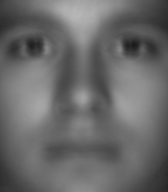
\includegraphics{src/beamer/figures/mean.jpg}
  \end{figure}
\end{frame}

\againframe<3->{calcul}




\begin{frame}
  \frametitle{Observations sur la Matrice de Covariance}
  La matrice de covariance $C$ est :
  \begin{itemize}
  \item<2-> symétrique réelle.
  \item<3-> définie semi-positive.
  \end{itemize}
\end{frame}



\subsection{Analyse en composantes principales}
\begin{frame}
  \frametitle{Introduction à l'Analyse en Composantes Principales}
  \begin{block}{Principe}
    Trouver des axes décrivant au mieux notre nuage de points.
  \end{block}
  \pause
  \begin{defi}[Eigenfaces]
    La méthode développéee par Turk et Pentland définit les \emph{eigenfaces} comme les axes principaux de l'ACP.
  \end{defi}
\end{frame}


% [[0.547824   0.07046611]
%  [0.07046611 0.12358077]]

%  [[ 0.98716928  0.15967719]
%  [-0.15967719  0.98716928]]

%  [[0.54524152]
%  [0.10937813]]


\begin{frame}
  \frametitle{Illustration en 2 Dimensions}
  \begin{figure}
    \begin{overprint}
      \only<1>{\centering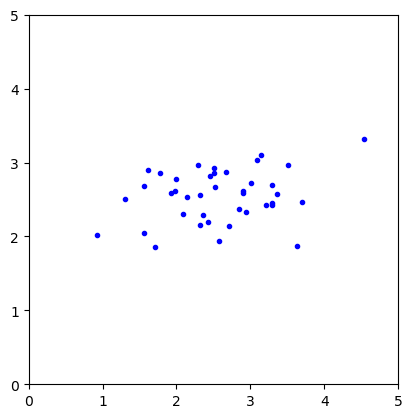
\includegraphics[scale=0.5]{src/beamer/figures/fig_pca_1.png}}
      \only<2>{\centering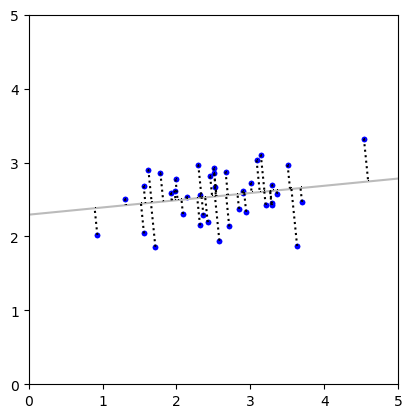
\includegraphics[scale=0.5]{src/beamer/figures/fig_pca_3.png}}
    \end{overprint}
  \end{figure}
\end{frame}



\begin{frame}
  \begin{figure}
    \frametitle{Lien avec la Matrice de Covariance}
    \begin{columns}
      \column{0.5\textwidth}
      \begin{align*}
        \onslide<1->{
        C &= 
            \begin{pmatrix}
              0.55 & 0.07\\
              0.07 & 0.12
            \end{pmatrix}                     
        \\}
        \onslide<2->{
          &= P
            \begin{pmatrix}
              0.55 & 0\\
              0    & 0.11
            \end{pmatrix}                     
                     P^T
                     }
      \end{align*}
      \onslide<2->{avec
      \[
        P =
        \begin{pmatrix}
          0.99 & -0.16\\
          0.16 & 0.99
        \end{pmatrix}
      \]}
      \column{0.5\textwidth}
      \begin{overprint}
        \onslide<1>\centering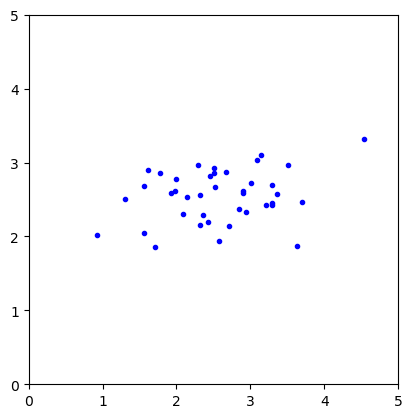
\includegraphics[scale=0.5]{src/beamer/figures/fig_pca_1.png}
        \onslide<2>\centering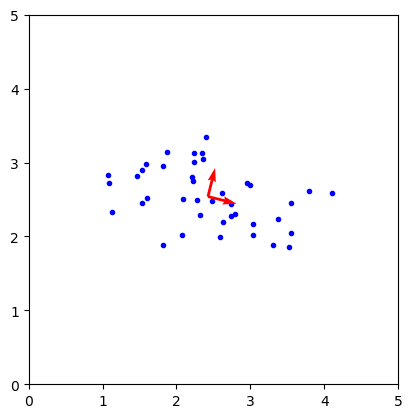
\includegraphics[scale=0.5]{src/beamer/figures/fig_pca_4.png}          
      \end{overprint}
    \end{columns}
  \end{figure}
\end{frame}



\begin{frame}
  \frametitle{Limite de la Méthode}
  \begin{qst}
    Quels sont les problèmes de la méthode ?
  \end{qst}

  \pause
  
  \begin{exampleblock}{Réponse}
    \begin{itemize}
    \item La matrice de covariance est de taille $N^2 \times N^2$.
      \pause
    \item La diagonaliser est infaisable informatiquement.
    \end{itemize}
  \end{exampleblock}
\end{frame}



\subsection{Décomposition en valeurs singulières}
\begin{frame}
  \frametitle{\'{E}noncé de la Décomposition en Valeurs Singulières}
  \begin{thm}
    Soit $M$ une matrice $m \times n$, alors il existe une décomposition de la forme
    \[
      M = U \Sigma V^t
    \]
    avec $U$ et $V$ des matrices orthonormales de taille respectives $m \times m$ et $n \times n$.
  \end{thm}
  
  \begin{prop}
    \begin{itemize}
    \item les colonnes de $V$ sont les vecteurs propres de $M^TM$
    \item les colonnes de $U$ sont les vecteurs propres de $MM^T$
    \end{itemize}
  \end{prop}
\end{frame}


\section{Classification des visages}
\subsection{Projection dans l'espace des visages}
\begin{frame}
  \frametitle{Projection d'un visage}
  Soit $\Gamma$ une nouvelle image de visage, on la projette dans l'espace des visages par :
  \[
    \omega_k = u_k^T(\Gamma - \Psi)
  \]
  
  \pause

  Pour $k \in \{1,\dotsc,M'\}$, on a alors :
  \[W =
    \begin{pmatrix}
      \omega_1 \\
      \vdots \\
      \omega_{M'}
    \end{pmatrix}
  \]
\end{frame}



\subsection{Analyse de la projection}
\begin{frame}
  \[
    \text{image reconstruite} = U \cdot \Gamma + \Psi
  \]
\end{frame}



\begin{frame}
  \frametitle{Conclusion de l'Analyse}
  \resizebox{\linewidth}{!}{
    \begin{tabular}{ | l | c | c | }
      \hline
                                      & proche d'une classe de visage & éloigné d'une classe de visage \\
      \hline
      proche de l'espace des visages  & \onslide<2->{visage connu}    & \onslide<3->{visage inconnu}   \\
      \hline
      éloigné de l'espace des visages & \onslide<4->{faux positif}    & \onslide<5->{pas un visage}    \\
      \hline
    \end{tabular}
  }
\end{frame}



\section{Application}
\subsection{Techniques utilisées aujourd'hui}

\begin{frame}
  \frametitle{Réseau de Neurones Convolutifs}

  \only<1>{
    \begin{block}{Principe}
      Reproduire le cortex visuel humain.
    \end{block}
    
    \centering\scalebox{0.4}{% Picture by Kroum Tzanev
\tikzset{
  pics/grid matrix/.style ={
    code = {
      \foreach[count=\i from 0] \l in {#1}
          \xdef\n{\i}; % \n va contenir le nombre de lignes
      \fill (0,0) rectangle (\n,\n); % rempli le fond
      \draw[draw grid/.try] (0,0) grid (\n,\n); % dessine la grille
      \draw[line width=1pt] (0,0) rectangle (\n,\n); % dessine la bord extérieur
      \foreach[count=\j] \l in {#1}
        \foreach[count=\i] \e in \l{
          % on place les nombres à l'intérieur de la grille
          \path ({\i-.5},{\n+.5-\j}) node[transform shape,M\i\j/.try] (-M\i\j){\e};
        }
    }
  },
  grid color/.style={
  	draw grid/.style=#1
  }
}

  \begin{tikzpicture}
    \def\xK{2}
    \def\yK{1}
    \def\zK{4}
\begin{scope}[yscale=1.3,xscale=.9,yslant=.35,nodes={font=\bfseries\sffamily\huge},z={([yslant=-.35]1,0)}]

    \def\zS{12}\pgfmathsetmacro\zKS{\zS-\zK}
    \path (0,0,0)
      pic[
        fill=blue!50!green!5,
        grid color=blue,
        draw=blue,
        transform shape
      ] (I)
      {
        grid matrix=
        {
          {, , , , , , },
          {, , , , , , },
          {, , , , , , },
          {, , , , , , },
          {, , , , , , },
          {, , , , , , },
          {, , , , , , },
        }
      }
    ;
    \draw[blue, ultra thick] (\xK,\yK,0) rectangle ++(3,3,0);
    % la connexion I -> K
%     \fill[opacity=.1,red] (\xK,\yK,0) -- ++(0,0,\zK) -- ++(3,0,0) -- ++(0,0,-\zK);
%     \fill[opacity=.1,red] (\xK,\yK,0) -- ++(0,0,\zK) -- ++(0,3,0) -- ++(0,0,-\zK);
%     \fill[opacity=.03,red] (\xK,\yK,0) ++(0,3,0) -- ++(0,0,\zK) -- ++(3,0,0) -- ++(0,0,-\zK);
% %     \draw (\xK,\yK,0) -- ++(0,0,\zK);
%     \draw (\xK+3,\yK,0) -- ++(0,0,\zK);
%     \draw (\xK,\yK+3,0) -- ++(0,0,\zK);
%     \draw (\xK+3,\yK+3,0) -- ++(0,0,\zK);

%     \path (\xK,\yK,\zK)
%       pic[
%         grid color=blue,
%         draw=blue,
%         fill=blue!5,
%         transform shape
%       ] (K)
%       {
%         grid matrix=
%         {
%           {1, 1, 0},
%           {0, 1, 0},
%           {2, 0, 1},
%         }
%       }
%     ;


  % inputs of the neuron
   \foreach\i in{1,2,3}{
      \foreach \j in {1,2,3}{
            \draw[ultra thick]  (\xK+1.5,\yK+1.5,\zK) -- (\xK-0.5+\i,\yK+\j-0.5,0);
  }}
  
    \draw[red!84!blue, ultra thick] (\xK+1,\yK+1,\zS) rectangle ++(1,1,0);

\shade[yscale=1/1.3,xscale=1/0.9,yslant=-0.45,ball color=blue!20!white,opacity=1] (\xK+0.5,\yK+5,\zK) circle (1);
  
  % outpus of the neuron
\draw[ultra thick,->,>=latex]  (\xK+2,\yK+1.35,\zK)--(\xK+1.5,\yK+1.5,\zS);

%     \fill[opacity=.1,blue] (\xK,\yK,\zK) -- ++(1,1,\zKS) -- ++(1,0,0) -- ++(1,-1,-\zKS);
%     \fill[opacity=.1,blue] (\xK,\yK,\zK) -- ++(1,1,\zKS) -- ++(0,1,0) -- ++(-1,1,-\zKS);
%     \fill[opacity=.03,blue] (\xK,\yK+3,\zK) -- ++(1,-1,\zKS) -- ++(1,0,0) -- ++(1,1,-\zKS) ;
%     \draw (\xK,\yK,\zK) -- ++(1,1,\zKS);
%     \draw (\xK,\yK+3,\zK) -- ++(1,-1,\zKS);
%     \draw (\xK+3,\yK,\zK) -- ++(-1,1,\zKS);
%     \draw (\xK+3,\yK+3,\zK) -- ++(-1,-1,\zKS);
    \path (0,0,\zS)
      pic[
        grid color=red,
        draw=red,
        fill=red!70!blue!7,
        fill opacity=.5,
        text opacity=1,
        transform shape
      ] (K)
      {
        grid matrix=
        {
          {, , , , , , },
          {, , , , , , },
          {, , , , , , },
          {, , , , , , },
          {, , , , , , },
          {, , , , , , },
          {, , , , , , },
        }
      }
    ;






\end{scope} 




\end{tikzpicture}}
  }

  \only<2>{
    \centering\scalebox{0.25}{
\begin{tikzpicture}[scale=1,yscale=1.3,xscale=0.9,yslant=.35,nodes={font=},z={([yslant=-.5]1,0)}]


%\begin{tikzpicture}[scale=0.5,yscale=1.3,xscale=0.9,yslant=.35,nodes={font=\bfseries\sffamily\huge},z={([yslant=-.5]1,0)}]


\xdef\filtersep{0.25};  % distance between two filter




%%%%%%%%%%%%%%%%%%
% Input image
\xdef\position{0};
\xdef\size{4};   % instead of 28x28
\xdef\numfilter{1};

\foreach \i in {1,...,\numfilter}{ 
  % \filldraw[thick, fill=gray] (-\halfsize,-\halfsize,\position+2*\i*\filtersep) rectangle (\halfsize,\halfsize,\position+2*\i*\filtersep);
  \filldraw[thick, fill=blue!20] (-\size/2,-\size/2,{\position+(2*\i+1)*\filtersep}) rectangle (\size/2,\size/2,{\position+(2*\i+1)*\filtersep});
}

% \fill[red] (-\size/2,-\size/2,\position+3*\filtersep) rectangle ++(1,1,0);
\node[above left=1ex]  at (\size/2,\size/2,1) {Entrée};
\node[below=3ex]  at (-\size/2,-\size/2,1) {$(28,28,1)$};


% Arrow
\draw[->, >=latex, gray!30, line width=4] (\size/2,\size/2,\position+2)  -- ++(0,0,5) node[midway, above=2ex, black,scale=0.7]{Convolution 32 couches};



%%%%%%%%%%%%%%%%%%
% Conv32
\xdef\position{8};
\xdef\size{4};
\xdef\numfilter{16};

\foreach \i in {1,...,\numfilter}{ 
  \filldraw[thick, fill=red!80!blue!20] (-\size/2,-\size/2,\position+2*\i*\filtersep) rectangle (\size/2,\size/2,\position+2*\i*\filtersep);
  \filldraw[thick, fill=red!60] (-\size/2,-\size/2,{\position+(2*\i+1)*\filtersep}) rectangle (\size/2,\size/2,{\position+(2*\i+1)*\filtersep});
}

\node[below=5ex] at (-\size/2,-\size/2,\position+\numfilter*\filtersep) {$(28,28,32)$};

% Arrow
\draw[->, >=latex, gray!30, line width=4] (\size/2,\size/2,\position+2*\numfilter*\filtersep+2)  -- ++(0,0,5) node[midway, above=2ex, black,scale=0.7]{Convolution 16 couches};



%%%%%%%%%%%%%%%%%%
% Conv16
\xdef\position{24};
\xdef\size{4};
\xdef\numfilter{8};

\foreach \i in {1,...,\numfilter}{ 
  \filldraw[thick, fill=green!80!blue!20] (-\size/2,-\size/2,\position+2*\i*\filtersep) rectangle (\size/2,\size/2,\position+2*\i*\filtersep);
  \filldraw[thick, fill=green!60!black!60] (-\size/2,-\size/2,{\position+(2*\i+1)*\filtersep}) rectangle (\size/2,\size/2,{\position+(2*\i+1)*\filtersep});
}

\node[below=5ex] at (-\size/2,-\size/2,\position+\numfilter*\filtersep) {$(28,28,16)$};

% Arrow
\draw[->, >=latex, gray!30, line width=4] (\size/2,\size/2,\position+2*\numfilter*\filtersep+1)  -- ++(0,0,4) node[midway, above=2ex, black,scale=0.7]{Aplatissement};

%%%%%%%%%%%%%%%%%%
% Vec grand
\xdef\position{36};
\xdef\size{4};

\filldraw[thick, fill=orange!80] (-0.25,-\size-2,\position) rectangle ++ (0.5,\size,0);
\filldraw[thick, fill=orange!80] (-0.25,2,\position) rectangle ++ (0.5,\size,0);

\foreach \i in {-1.5,-1,...,1.5}{
\fill[orange!80] (0,\i,\position) circle(0.15);
}

\node[below=3ex] at (0,-\size-2,\position) {vecteur $12544$};

% Arrow
\draw[->, >=latex, gray!30, line width=4] (\size/2,\size/2,\position-1)  -- ++(0,0,4) node[midway, above=2ex, black,scale=0.7]{Dense};

%%%%%%%%%%%%%%%%%%
% Vec10
\xdef\position{42};
\xdef\size{6};

\filldraw[thick, fill=cyan!80] (-0.25,-\size/2,\position) rectangle ++ (0.5,\size,0);

\node[below=3ex] at (0,-\size/2,\position) {$10$ neurones};
\node[below right=1ex]  at (0.5,\size/2,\position) {Sortie};


% Arrows
% \usetikzlibrary{3d}
%\begin{scope}[canvas is xz plane at y=-\size, transform shape]
%\pgflowlevelsynccm
%\draw[->, >=latex, gray!30, line width=0.5em] (\size/2,\size/2,3)  -- ++(0,10,0);
%\end{scope}

 \end{tikzpicture}}
  }
  
\end{frame}


\subsection{Les besoins auxquels répondent les technologies de reconnaissance faciale}
\begin{frame}
  \frametitle{Authentification et Identification}
  \begin{defi}[Authentification]
    Vérifier qu’une personne est bien celle qu’elle prétend être.
  \end{defi}
  
  \pause

  \begin{defi}[Identification]
    Retrouver une personne au sein d’un groupe d’individus, dans un lieu, une image ou une base de données.
  \end{defi}
\end{frame}



\subsection{Secteurs utilisant la reconnaissance faciale}
\begin{frame}
  \frametitle{Quelques Exemples}
  Identification :
  \begin{itemize}
  \item <2-> Facebook avec les suggestions.
  \item <4-> Traitement des antécédents judiciaires.
  \item <5-> Sécurité sur la voie publique.
  \end{itemize}

  Authentification :
  \begin{itemize}
  \item <3-> Accès à des services de retrait d'argents.
  \end{itemize}  
\end{frame}



\section{Conclusion}
\begin{frame}
\end{frame}



\subsection{Références}
\begin{frame}  
\end{frame}

\end{document}